\documentclass[tikz,border=10pt]{standalone}
\begin{document}
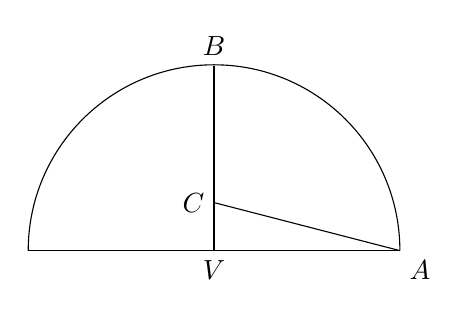
\begin{tikzpicture}[scale=1.0]
  \coordinate (V) at (0,0);
  \coordinate (A) at (2.36,0);
  \coordinate (B) at (0,2.35);
  \coordinate (C) at (0,0.61);

  \draw (-2.36,0) -- (A);
  \draw (V) -- (B);
  \draw (C) -- (A);
  \draw (-2.36,0) arc (180:0:2.36);

  \node[above] at (B) {$B$};
  \node[left] at (C) {$C$};
  \node[below] at (V) {$V$};
  \node[below right] at (A) {$A$};
\end{tikzpicture}
\end{document}
